\documentclass[tikz,border=4pt]{standalone}
\usepackage[scaled=0.92]{helvet}
\renewcommand{\familydefault}{\sfdefault}
\usepackage{amsmath,amssymb}
\usetikzlibrary{positioning,arrows.meta,calc,fit,backgrounds,shapes.geometric,decorations.pathreplacing}

% ---- palette ----
\definecolor{ink}{HTML}{1F2328}
\definecolor{muted}{HTML}{6B6A66}
\definecolor{line}{HTML}{C9C7C0}
\definecolor{paper}{HTML}{F7F6F2}
\definecolor{blue}{HTML}{2A78D6}
\definecolor{blueL}{HTML}{E4EEFA}
\definecolor{orange}{HTML}{EB6834}
\definecolor{orangeL}{HTML}{FCE9E1}
\definecolor{aqua}{HTML}{1BAF7A}
\definecolor{aquaL}{HTML}{E0F4EC}
\definecolor{violet}{HTML}{6250D6}
\definecolor{violetL}{HTML}{ECE9FA}
\definecolor{amber}{HTML}{C98500}
\definecolor{amberL}{HTML}{FBF1DC}

\tikzset{
  >={Stealth[length=5pt,width=4pt]},
  panel/.style={draw=line, line width=0.6pt, rounded corners=6pt, fill=paper},
  card/.style={draw=line, line width=0.5pt, rounded corners=4pt, fill=white},
  stage/.style={draw=#1, line width=0.7pt, rounded corners=4pt, fill=#1!8, minimum height=9mm, align=center, font=\scriptsize\color{ink}},
  chip/.style={rounded corners=2pt, fill=#1, text=white, font=\tiny\bfseries, inner sep=2pt, minimum height=3.6mm},
  stepn/.style={circle, fill=ink, text=white, font=\tiny\bfseries, inner sep=0.6pt, minimum size=3.6mm},
  flow/.style={->, line width=0.8pt, color=ink},
  soft/.style={->, line width=0.6pt, color=muted, dashed},
  title/.style={font=\footnotesize\bfseries\color{ink}, anchor=north west},
  sub/.style={font=\tiny\color{muted}, anchor=north west},
}


\begin{document}
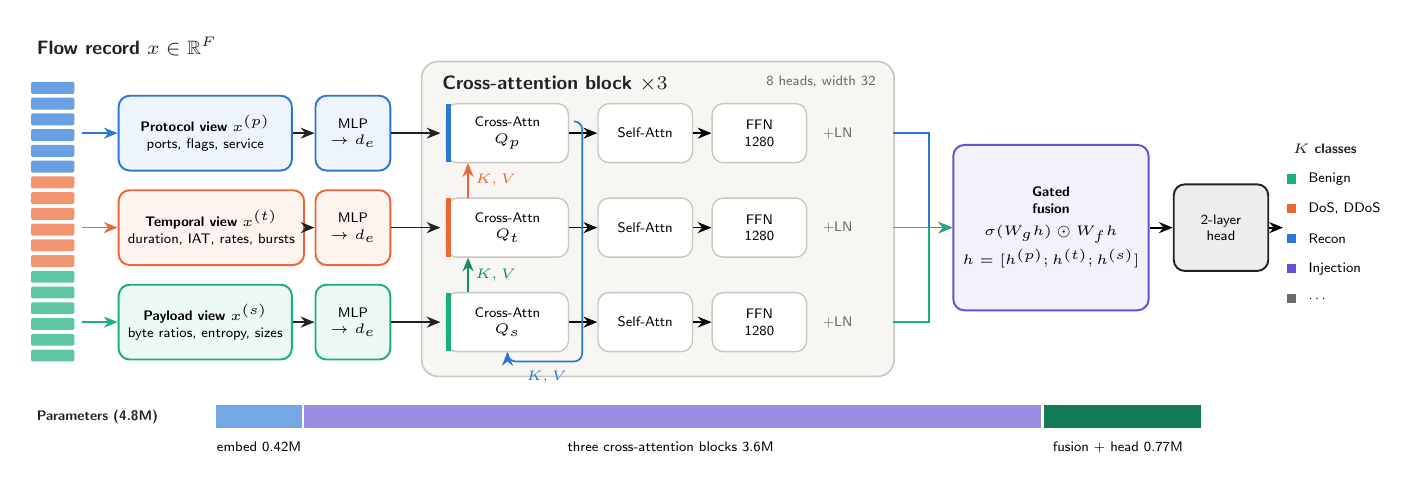
\begin{tikzpicture}[x=1cm,y=1cm]
% input flow vector
\node[font=\scriptsize\bfseries\color{ink}, anchor=west] at (0,4.55) {Flow record $x\in\mathbb{R}^F$};
\foreach \i in {0,...,17}{
  \pgfmathtruncatemacro{\g}{\i<6 ? 1 : (\i<12 ? 2 : 3)}
  \ifnum\g=1 \def\cc{blue}\fi \ifnum\g=2 \def\cc{orange}\fi \ifnum\g=3 \def\cc{aqua}\fi
  \fill[\cc!70, rounded corners=0.5pt] (0.05,3.95-\i*0.2) rectangle ++(0.55,0.15);
}
% views
\foreach \yy/\c/\nm/\ex/\tg in {3.45/blue/Protocol view $x^{(p)}$/{ports, flags, service}/p, 2.25/orange/Temporal view $x^{(t)}$/{duration, IAT, rates, bursts}/t, 1.05/aqua/Payload view $x^{(s)}$/{byte ratios, entropy, sizes}/s}{
  \draw[->, line width=0.6pt, color=\c] (0.7,\yy) -- (1.15,\yy);
  \node[stage=\c, minimum width=2.2cm, minimum height=0.95cm, anchor=west, font=\tiny] (v\tg) at (1.15,\yy) {\textbf{\nm}\\\ex};
  \node[stage=\c, minimum width=0.95cm, minimum height=0.95cm, anchor=west, font=\tiny] (e\tg) at (3.65,\yy) {MLP\\$\to d_e$};
  \draw[->, line width=0.6pt, color=ink] (v\tg) -- (e\tg);
}
% blocks
\node[panel, minimum width=6.0cm, minimum height=4.0cm, anchor=south west] (blk) at (5.0,0.35) {};
\node[font=\scriptsize\bfseries\color{ink}, anchor=north west] at (5.15,4.3) {Cross-attention block $\times 3$};
\node[font=\tiny\color{muted}, anchor=north east] at (10.9,4.3) {8 heads, width 32};
\foreach \yy/\c/\tg in {3.45/blue/p, 2.25/orange/t, 1.05/aqua/s}{
  \draw[->, line width=0.6pt, color=ink] (e\tg.east) -- (5.25,\yy);
  \node[card, minimum width=1.55cm, minimum height=0.75cm, font=\tiny, align=center] (ca\tg) at (6.1,\yy) {Cross-Attn\\$Q_{\tg}$};
  \node[card, minimum width=1.2cm, minimum height=0.75cm, font=\tiny, align=center] (sa\tg) at (7.85,\yy) {Self-Attn};
  \node[card, minimum width=1.2cm, minimum height=0.75cm, font=\tiny, align=center] (ff\tg) at (9.3,\yy) {FFN\\1280};
  \draw[->, line width=0.5pt] (ca\tg) -- (sa\tg);
  \draw[->, line width=0.5pt] (sa\tg) -- (ff\tg);
  \fill[\c] (5.32,\yy-0.37) rectangle ++(0.06,0.74);
}
% K,V routing p<-t, t<-s, s<-p
\draw[->, line width=0.6pt, color=orange, rounded corners=3pt] (5.6,2.25+0.38) -- (5.6,3.45-0.38) node[midway, right=-1pt, font=\tiny] {$K,V$};
\draw[->, line width=0.6pt, color=aqua!80!black, rounded corners=3pt] (5.6,1.05+0.38) -- (5.6,2.25-0.38) node[midway, right=-1pt, font=\tiny] {$K,V$};
\draw[->, line width=0.6pt, color=blue, rounded corners=3pt] (6.95,3.45+0.15) -- (7.05,3.45+0.15) -- (7.05,0.55) -- (6.1,0.55) -- (6.1,1.05-0.38);
\node[font=\tiny\color{blue}, anchor=north] at (6.6,0.55) {$K,V$};
\node[font=\tiny\color{muted}, anchor=west] at (9.95,3.45) {\,+LN};
\node[font=\tiny\color{muted}, anchor=west] at (9.95,2.25) {\,+LN};
\node[font=\tiny\color{muted}, anchor=west] at (9.95,1.05) {\,+LN};
% fusion
\foreach \yy/\c/\tg in {3.45/blue/p, 2.25/orange/t, 1.05/aqua/s}{
  \draw[->, line width=0.6pt, color=\c] (11.0,\yy) -- (11.45,\yy) -- (11.45,2.25) -- (11.75,2.25);
}
\node[stage=violet, minimum width=2.45cm, minimum height=2.1cm, anchor=west, font=\tiny] (fu) at (11.75,2.25) {\textbf{Gated}\\\textbf{fusion}\\[2pt]$\sigma(W_g h)\odot W_f h$\\[1pt]$h=[h^{(p)};h^{(t)};h^{(s)}]$};
\node[stage=ink, minimum width=1.2cm, minimum height=1.1cm, anchor=west, font=\tiny] (hd) at (14.55,2.25) {2-layer\\head};
\draw[->, line width=0.7pt] (fu) -- (hd);
% output classes
\foreach \c/\n [count=\i] in {aqua/Benign, orange/{DoS, DDoS}, blue/Recon, violet/Injection, muted/\dots}{
  \node[font=\tiny, anchor=west] at (16.15,3.25-\i*0.38) {\n};
  \fill[\c] (16.0,3.25-\i*0.38-0.06) rectangle ++(0.12,0.12);
}
\draw[->, line width=0.7pt] (hd) -- (15.95,2.25);
\node[font=\tiny\bfseries\color{ink}, anchor=west] at (15.95,3.25) {$K$ classes};

% parameter budget bar
\node[font=\tiny\bfseries\color{ink}, anchor=west] at (0,-0.15) {Parameters (4.8M)};
\fill[blue!65] (2.4,-0.3) rectangle ++(0.42*2.6,0.3);
\fill[violet!65] (2.4+0.42*2.6+0.03,-0.3) rectangle ++(3.6*2.6,0.3);
\fill[aqua!70!black] (2.4+4.02*2.6+0.06,-0.3) rectangle ++(0.77*2.6,0.3);
\node[font=\tiny, anchor=north] at (2.4+0.21*2.6,-0.35) {embed 0.42M};
\node[font=\tiny, anchor=north] at (2.4+0.42*2.6+1.8*2.6,-0.35) {three cross-attention blocks 3.6M};
\node[font=\tiny, anchor=north] at (2.4+4.02*2.6+0.385*2.6,-0.35) {fusion + head 0.77M};
\end{tikzpicture}
\end{document}
